% 2002 年春季上海卷第 19 题：三棱柱空间图形
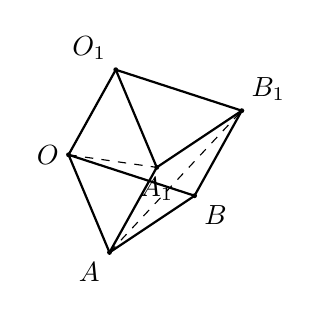
\begin{tikzpicture}[>=stealth, scale=0.8]
  \coordinate (O) at (0,0);
  \coordinate (B) at (2.0,-0.65);
  \coordinate (A) at (0.65,-1.55);
  \coordinate (Oone) at (0.75,1.35);
  \coordinate (Bone) at (2.75,0.70);
  \coordinate (Aone) at (1.4,-0.20);

  \draw[thick] (O)--(B)--(A)--cycle;
  \draw[thick] (Oone)--(Bone)--(Aone)--cycle;
  \draw[thick] (O)--(Oone) (B)--(Bone) (A)--(Aone);
  \draw[dashed] (O)--(Aone) (A)--(Bone);

  \fill (O) circle (1.1pt) node[left] {$O$};
  \fill (B) circle (1.1pt) node[below right] {$B$};
  \fill (A) circle (1.1pt) node[below left] {$A$};
  \fill (Oone) circle (1.1pt) node[above left] {$O_1$};
  \fill (Bone) circle (1.1pt) node[above right] {$B_1$};
  \fill (Aone) circle (1.1pt) node[below] {$A_1$};
\end{tikzpicture}
